\section{Approach Overview}
\eat{总分结构}
We realize our strategy as a framework/tool, \toolname, of which workflow is shown in Figure~\ref{fig:workflow}. The input of \toolname is \blank{}. The output of \toolname is \blank{}. \toolname has \blank{} components/steps. The first component is \blank{}, which accepts \blank{} and outputs \blank{}. Intuitively, the first component does \blank{}. We do this because \blank{}. The second component is \blank{}, which accepts \blank{} and outputs \blank{}. Intuitively, the second component does \blank{}. We do this because \blank{}. The third component is \blank{}, which accepts \blank{} and outputs \blank{}. Intuitively, the third component does \blank{}. We do this because \blank{}. 

\begin{figure*}[t!]
    \centering
    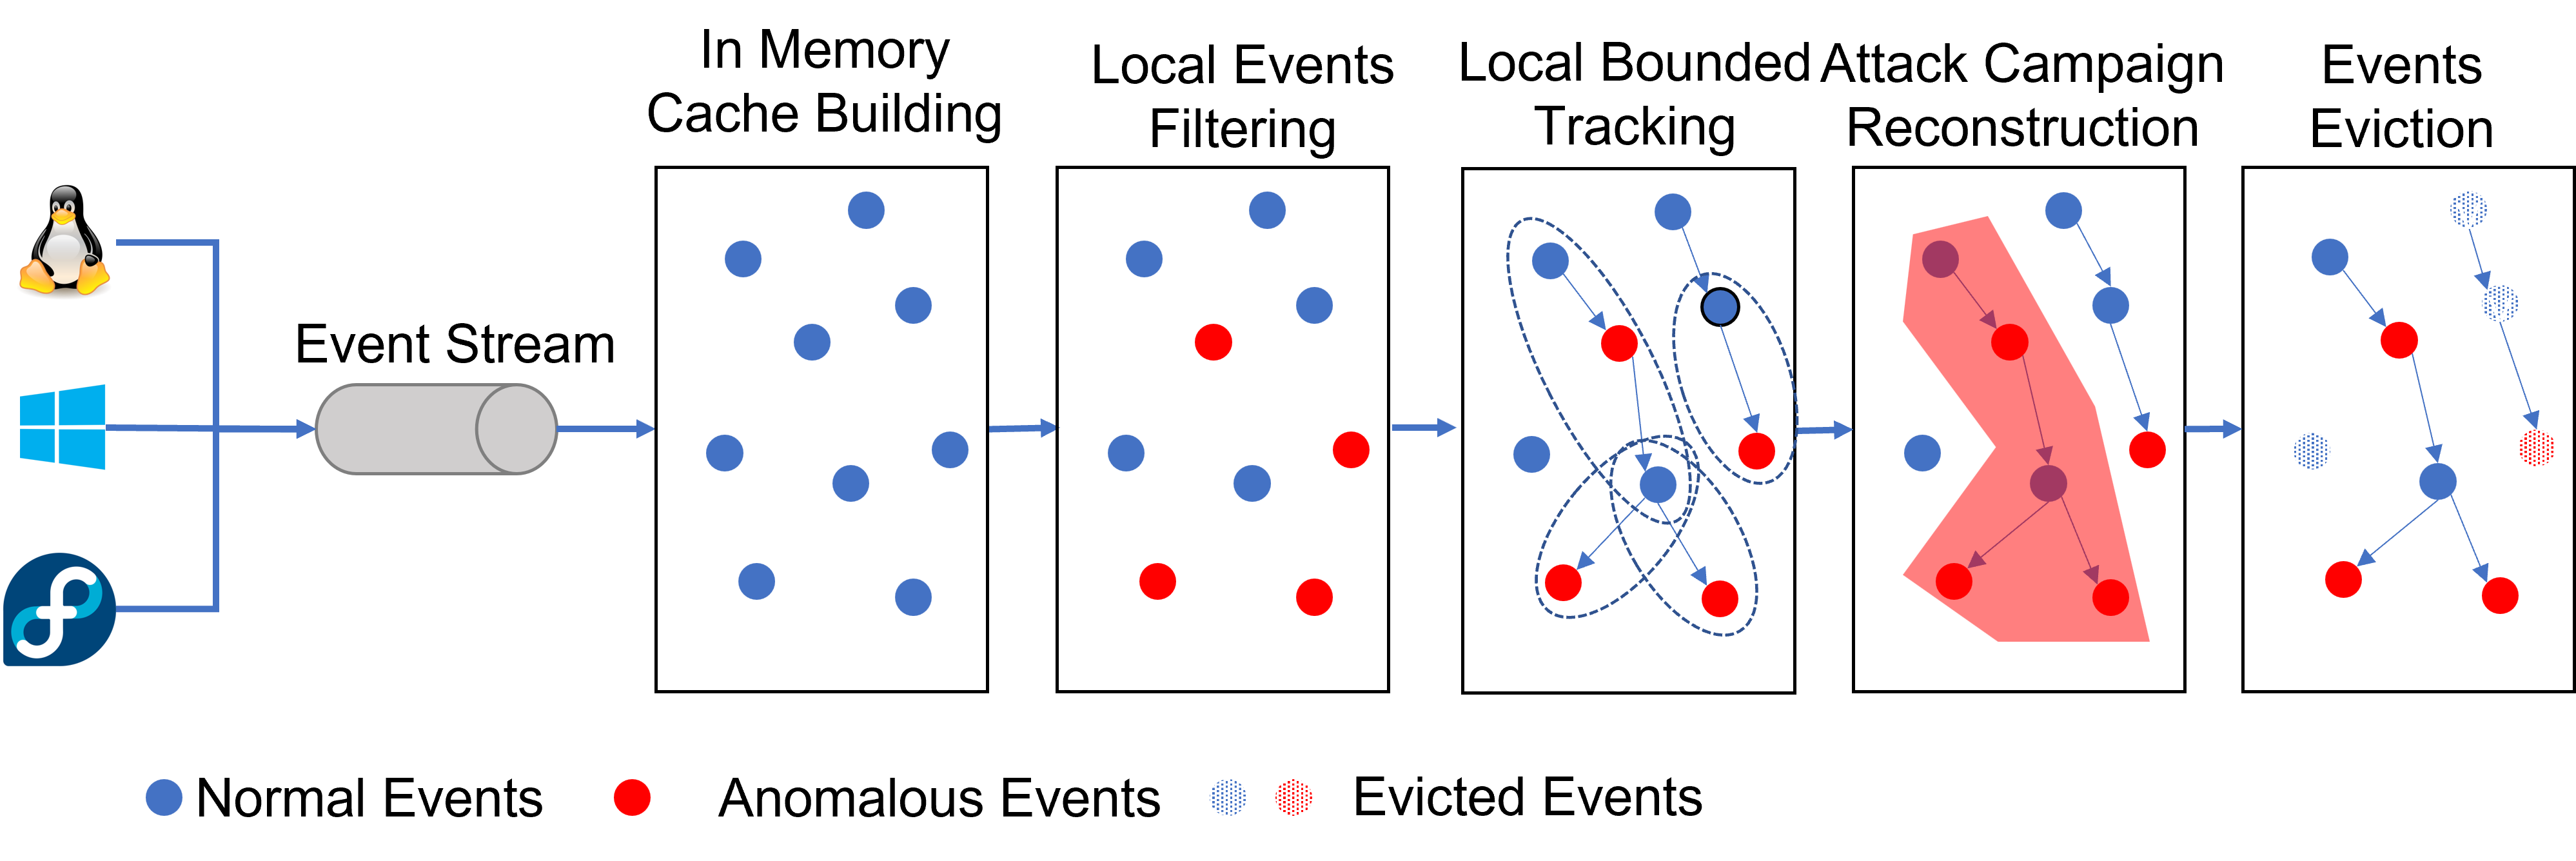
\includegraphics[width=\textwidth]{fig/workflow.png}
	\caption{Your beaultiful workflow picture}
	\label{fig:workflow}
\end{figure*}
\section{Design}
In this section, we discuss the design details of the components of \toolname. 
\explain{I will make an example for one component, add more based on your need}
\subsection{Component 1}
The goal of \blank{the name of component 1} is \blank{}. We use  \blank{the name of component 1} because \blank{}. 

On the high-level, \blank{the name of component 1} is a \blank{}.However, to address our technical problem, we need to address \blank{} engineering problems, which are \blank{}, \blank{}, and \blank{}. 

\explain{There are some examples}
To address the engineering/technical problem \blank{}, we leverage a data structure \blank{}. This data structure is a graph whose nodes are \blank{} and edges are \blank{}. This graph is an attributed graph. Therefore, each node has an attribute that represents \blank{}. Formally, we define the graph as \blank{your mathematical equations}.

To address the engineering/technical problem \blank{}, we leverage a deep learning model \blank{}. We choose this deep learning model \blank{} because it can \blank{}. The deep learning model consists of \blank{} components, which are \blank{}. Formally, the deep learning model is \blank{your math}.We choose this deep learning model \blank{} because it can \blank{}. The deep learning model consists of \blank{} components, which are \blank{}. Formally, the deep learning model is \blank{your math}.



To address the engineering/technical problem \blank{}, we propose a heuristic algorithm. On the high level, our algorithm does \blank{}. The formal pseudocode is in Algorithm~\ref{}. Specifically, \blank{discuss the critical steps in the Algorithm}

